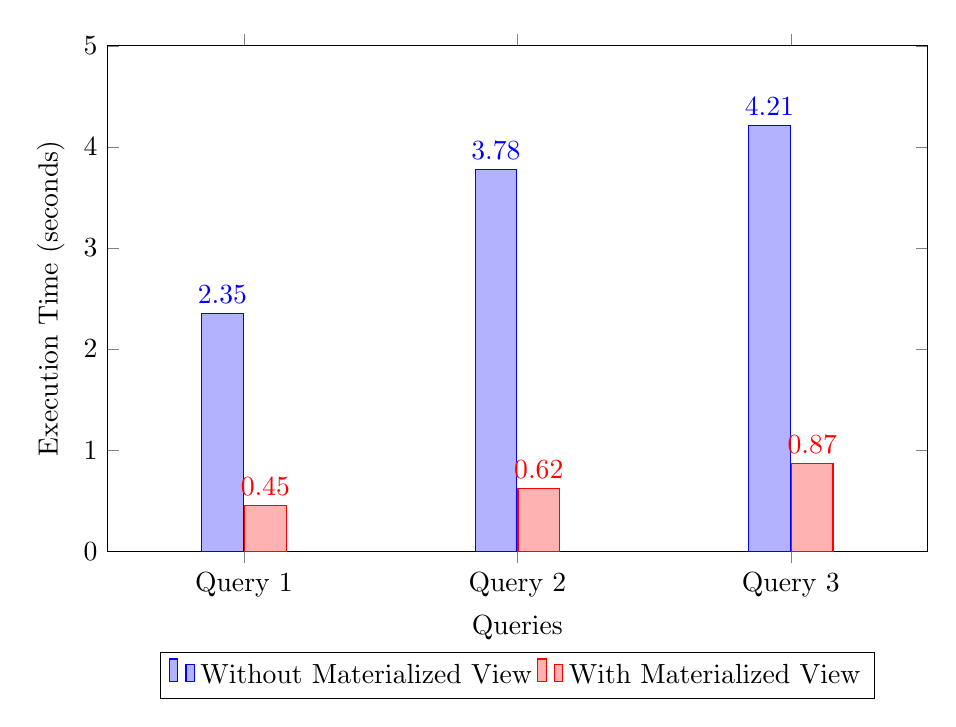
\begin{tikzpicture}
    \begin{axis}[
        width=12cm, height=8cm,
        ybar=0.5pt, % Bar style
        bar width=15pt,
        symbolic x coords={Query 1, Query 2, Query 3},
        xtick=data,
        ymin=0, ymax=5,
        ylabel={Execution Time (seconds)},
        xlabel={Queries},
        legend style={at={(0.5,-0.2)}, anchor=north, legend columns=-1},
        nodes near coords, % Show data labels
        enlarge x limits=0.25
    ]
        % Without Materialized View Data
        \addplot coordinates {(Query 1,2.35) (Query 2,3.78) (Query 3,4.21)};
        % With Materialized View Data
        \addplot coordinates {(Query 1,0.45) (Query 2,0.62) (Query 3,0.87)};
        
        \legend{Without Materialized View, With Materialized View}
    \end{axis}
\end{tikzpicture}